\chapter{Relativistic Spacetime}
\label{chapter:relativistic_spacetime}

%\section*{Objectives}
%\begin{objectives}
%\item Be able to calculate a spacetime interval between two events,
%  and classify the interval as space-like, time-like or light-like.
%  Use these classifications to determine whether or not the two events
%  could be causally linked.
%\item Be able to use the invariance of the interval to relate distance
%  and time intervals in one reference frame to those in a different
%  frame.
%\item Be able to draw and/or interpret a spacetime diagram, and use
%  this diagram to determine temporal and spatial ordering of events,
%  including whether or not events are simultaneous or at the same
%  location.
%\end{objectives}

\section{Introduction}


The previous chapter introduced the basic ideas of relativity along
with some of the most dramatic implications of the theory.  But the
predictions of time dilation and length contraction are merely special
cases of a much broader theory.  In this chapter, we discuss the idea
of spacetime, which blends time and space together.  We introduce the
spacetime interval, a quantity that is one of the fundamental
invariants in relativity, and we use this interval to relate distance
and time measurements made in different reference frames that 
are moving with respect to each other.  We also introduce
spacetime diagrams, which provide a graphical way of illustrating
relativistic phenomena, particularly the relativity of simultaneity.
    
%We also develop the relativistic velocity transformation formulas,
%which allow us to compute a particle's velocity in one inertial frame
%if we know the particle's velocity in another inertial frame.

\section{Spacetime intervals}

\label{sec:spacetime_intervals}

As we saw in Chapter \ref{chapter:relativityI}, observers in different reference frames
disagree about time and distance measurements.  But there are a few
quantities referred to as invariants upon which all observers agree
regardless of their reference frames.  One of these invariants was
discussed in the previous chapter; namely, the invariance of the speed
of light in a vacuum.  It turns out that distance and time can be
folded together to make another invariant, referred to as the
invariant spacetime interval $I$, defined by

\begin{equation}
I^2 \equiv \left(c\Delta t\right)^2 - \left(\Delta x\right)^2.
\label{eq:intervaldef}
\end{equation}
Note that $I^2$ can be positive, zero, or negative.  If $I^2$ is
positive, then the interval is called {\em time-like\/}  since the first term
--- with $\Delta t$ in it --- dominates.  Similarly, negative values
of $I^2$ correspond to {\em space-like\/} intervals, and if $I^2 = 0$, the
interval is called {\em light-like\/}.  Qualitatively, an event is light-like
if a pulse of light could travel directly between the two events.
This can be seen from Eq.~(\ref{eq:intervaldef}): if $I^2 = 0$, then
\begin{align}
0 &= \left(c\Delta t\right)^2 - \left(\Delta x\right)^2  \nonumber \\
\Rightarrow \Delta x &= \pm c \Delta t,
\end{align}
as would be expected for a pulse of light traveling a distance $\Delta
x$ in a time $\Delta t$.

Two events could be {\em causally-linked} (i.e., event A actually
causes or contributes to event B) if the spacetime interval between
them is either light-like or time-like.  In fact, for time-like
spacetime intervals, the interval is the proper time (multiplied by $c$).  
If two events are separated by a space-like interval, then no 
information can travel between the two events since it would require 
superluminal ($|v| > c$) information transmission, and nothing 
(especially information) can travel faster than light relative to 
any observer.  So events {\em can't} be causally linked if the square 
of the spacetime interval between them is negative.


\begin{example}{Causality and intervals}  
  In the year 2055, a father and his daughter are watching the 5$^{\rm
    th}$ game of the National League Divisional Series from a Moon base at the Sea of
  Tranquility.  The Washington Nationals lead the St. Louis Cardinals by a run with 2 outs 
  in the bottom of the ninth
  inning, but the bases are loaded. The daughter sneezes and then watches in horror as
  $2.0\units{s}$ later Drew Storen, Jr., of the Nationals throws
  a wild pitch that not only walks in the tying run but also allows St. Louis to
  score the winning run. Distraught, the
  daughter bursts into tears. ``What's wrong?'' her father asks.
  ``It's my fault that the Nats lost!  My sneeze caused Storen to throw
  that wild pitch!'' What argument should the father use to assure his daughter
  that she is not personally responsible for yet another
  heart-breaking Nats playoff loss?  

\solution The father should first point
  out that the distance between the Earth and Moon is $3.84\times
  10^8\units{m}$, or $1.3\units{lt-s}$.  So, if the father/daughter
  received the TV signal of the strikeout $2.0\units{s}$ after the
  sneeze, in their reference frame it must have actually occurred only
  $0.7\units{s}$ after the sneeze.  (It takes the TV signal
  $1.3\units{s}$ to make it from the Earth to the Moon.)  Now, the
  father should calculate the spacetime interval:
\begin{align}
I^2 &= \left(c\Delta t\right)^2 - \left(\Delta x\right)^2 % \nonumber \\
    = (1\units{lt-s/s}\times 0.7\units{s})^2 - 
                    (1.3\units{lt-s})^2 % \nonumber \\
    = -1.2\, (\mbox{lt-s})^2 \nonumber 
\end{align}
So, the father should pat the daughter on the head and say, ``So,
you see honey ---  you can't have caused Storen to throw that wild pitch 
because the spacetime interval between your sneeze and his strikeout
is a space-like interval!''\footnote{By the way, we originally wrote this
problem about the Red Sox when they hadn't won a World Series in over 80
years. The following year, they won the World Series. And {\bf that} is a
{\em time-like} interval, so, yes, we do take credit for the Red
Sox victory.}
\footnote{And then we switched the example to one with the Cubs because,
well, it didn't work for the Red Sox anymore, and we figured, "Well, we'll be
able to use this example for {\bf decades} because the Cubs will never win
the World Series!" But the Cubs messed that up this past year. (Also a
time-like interval, so we take credit for the Cubs World Series
championship, too.) Fans of
the Nationals in PHYS 211 requested that we use the Nats now in this example.}
\label{example:causality-intervals}
\end{example}

Don't worry about the fact that $I^2$ is negative for space-like
intervals.  The definition of $I^2$ in Eq.~(\ref{eq:intervaldef}) is
chosen so that for time-like intervals, the interval $I$ itself is the
proper time (multiplied by $c$), which is convenient for our purposes.  
But the interval could have equally been defined as 
$I^2 = \left(\Delta x\right)^2 - \left(c \Delta t\right)^2$, 
in which case $I^2$ would be negative for
time-like intervals (some authors do, in fact, define $I^2$ this way).
In fact, some physicists define two different intervals: $I^2 =
\left(c\Delta t\right)^2-\left(\Delta x\right)^2$ for time-like
intervals and $I^2 = \left(\Delta x\right)^2-\left(c\Delta t\right)^2$
for space-like intervals.  We will stick with Eq.~(\ref{eq:intervaldef}).

As stated earlier, $I^2$ is an invariant --- observers in different
reference frames will agree on the value of this interval for any two
events:
    
\begin{equation}
I^2 = \left(I^\prime\right)^2,
\end{equation}
or

\begin{boxiteq}{
\begin{equation}
\left(c\Delta t\right)^2 - \left(\Delta x\right)^2 = 
              \left(c\Delta t^\prime\right)^2 - 
     \left(\Delta x^\prime\right)^2.
\label{eq:interval-invariance}
\end{equation}
}
\end{boxiteq}

\noindent This is important for several reasons.  First, the
invariance of the interval helps to further clarify the intimate
connection between distance and time in relativity.  Any disagreements
between different observers about the time interval between events
must be accompanied by a corresponding disagreement in the distance in
order to keep the interval invariant.  Second, if an interval is
space-like or time-like or light-like as viewed in one reference
frame, then it is the same kind of interval as viewed in any reference
frame.  This makes sense: if two events cannot be causally-linked in
one reference frame, for instance, it would be nonsensical to think
that they would be causally-linked as observed by someone in a
different reference frame.  Finally, the interval can be used to
determine how events are viewed in one reference frame, given
information in a different frame.  As an example, we refer back to a
problem from the previous chapter.


\begin{example}{Using the interval} 
  A spaceship crew wants to make the trip from Earth to Alpha Centauri
  in only 2.0 years as measured by clocks on board their spaceship.\\
  (a) How long does the trip take according to Earth-frame observers?
  (b) How fast must the astronauts travel relative to Earth?
  \solution For problem \ref{prob:alpha_centauri} in
  chapter~\ref{chapter:relativityI}, you used the proper time relation,
  but you had to express the speed in terms of the unknown travel time
  according to Earth-frame observers.  Here, we do the same problem
  but using the spacetime interval.

  \noindent (a) We know that the distance to Alpha Centauri is 
  $4\units{lt-yr}$ as measured by observers on the Earth, so $\Delta x =
  4\units{lt-yr}$.  From the statement of the problem, we can see that
  $\Delta t^\prime = 2\units{yr}$.  And since the astronauts are
  present both at the launching of the rocket and its arrival at Alpha
  Centauri, it follows that $\Delta x^\prime = 0$.  Using the
  interval, we have
\begin{align}
\left(c\Delta t\right)^2 - \left(\Delta x\right)^2 &= 
   \left(c\Delta t^\prime\right)^2 -\left(\Delta x^\prime\right)^2 \nonumber \\
\Rightarrow \left(c\Delta t\right)^2 &= \left(c\Delta t^\prime\right)^2 - 
     \left(\Delta x^\prime\right)^2 + \left(\Delta x\right)^2 \nonumber \\
\Rightarrow \left(\Delta t\right)^2 &= (2\units{y})^2 + 
                         \frac{(4\units{lt-yr})^2}{(1\units{lt-yr/yr})^2} - 0^2
                                                          \nonumber \\
                                  &= 20\units{y}^2    \nonumber \\
\Rightarrow \Delta t &= 4.47\units{y}. \nonumber
\end{align}
(b) The speed of the astronauts' ship is then simply
\begin{equation}
  v = \frac{\Delta x}{\Delta t} =
  \frac{4\units{lt-yr/yr}}{4.47\units{y}}  
   = 0.89\units{lt-yr/yr} = 0.89c.
\end{equation}
\label{example:intervals-causality}
\end{example}

As you might have guessed from this example, the relations from the
previous chapter (time dilation and length contraction) are both
special cases of the more general invariance of the spacetime
interval.  The proper time relation, Eq.~(\ref{eq:ptr}) corresponds to
a situation where one of the observers is at both events.  Let's say
that the observer in the primed reference frame is at both events
(i.e., measures the proper time).  Then $\Delta x^\prime = 0$.  The
distance $\Delta x$ (the distance between events as measured by the observer
in the unprimed frame) is simply $\Delta x = v\Delta t$ 
(distance = speed $\times$ time).
Eq.~(\ref{eq:interval-invariance}) then becomes:
\begin{eqnarray}
&&\left(c\Delta t\right)^2 - \left(v\Delta t\right)^2 = 
       \left(c\Delta t^\prime\right)^2 -  0^2 \nonumber \\
\Rightarrow &&\left(\Delta t\right)^2\left(1-v^2/c^2\right) = 
       \left(\Delta t^\prime\right)^2 \nonumber \\
\Rightarrow &&\Delta t^\prime = \Delta t\sqrt{1-v^2/c^2}, \nonumber 
\end{eqnarray}
which is, in fact, the proper time relation Eq.~(\ref{eq:ptr}) with
$\Delta t^\prime$ as the proper time (since the primed observer is at
both events) and with $\Delta t$ as the two-clock time.  Similar
arguments can be used to show that the length contraction relation,
Eq.~(\ref{eq:lengthcontract}), is a special case of the invariance of
the spacetime interval for situations where $\Delta t$ or $\Delta
t^\prime$ is zero.

\section{World Lines and Spacetime Diagrams}
\label{section:worldlines}

The motions of particles, clocks, or whatever can be represented on a
spacetime diagram.  A spacetime diagram consists of a pair of
perpendicular axes, with the vertical axis representing time and the
horizontal axis representing $x$ position in a particular inertial
reference frame.  The $x$-axis is the direction of relative motion
between this unprimed frame and another inertial frame called the
primed frame.
    
A plot of an object's position vs.\ time on a spacetime diagram is
called the {\em world line} of the object.  Three world lines are
shown in Fig.~\ref{fig:spacetime-example}; a straight world line
represents motion with constant velocity while a curved world line
represents accelerated motion.  An {\em event} is represented by a dot
on the spacetime diagram.
    
When drawing a spacetime diagram, make sure you use appropriate units.
(Do {\em not} use meters for length!)  For time (which we use as the
vertical axis on a spacetime diagram), we choose something appropriate
to the time scale of the problem, like years, seconds, nanoseconds,
etc.  Then we must choose an appropriate unit of distance equal to
that traveled by light in the chosen unit of time.  For example,
suppose we choose one second as the unit of time, then we would used
one lt-s (the distance traveled by light in one second) as the unit of
distance.  In these units the speed of light is $c = 
(1\units{lt-s})/(1\units{s}) = 1\units{lt-s/s}$.  In this method of
handling the units, the world line for a pulse of light must have a
slope that is numerically equal to $+1$ or $-1$.  {\bf And no world line 
can ever have a slope with magnitude less than 1; that would
correspond to an object traveling faster than light.}  Slopes can also
be used to determine if the interval between two events is time-like,
light-like or space-like.  If a line were to be drawn connecting the
two events, a time-like interval would correspond to a slope with
magnitude greater than 1, a light-like interval would correspond to a
slope with magnitude 1, and space-like interval would correspond to a
slope with magnitude less than 1 (note that in this last case, that
the ``line'' drawn between the two events can't be the world line
of any real object, since nothing can travel faster than $c$).
    
\begin{figure}[tbp]
\begin{center}
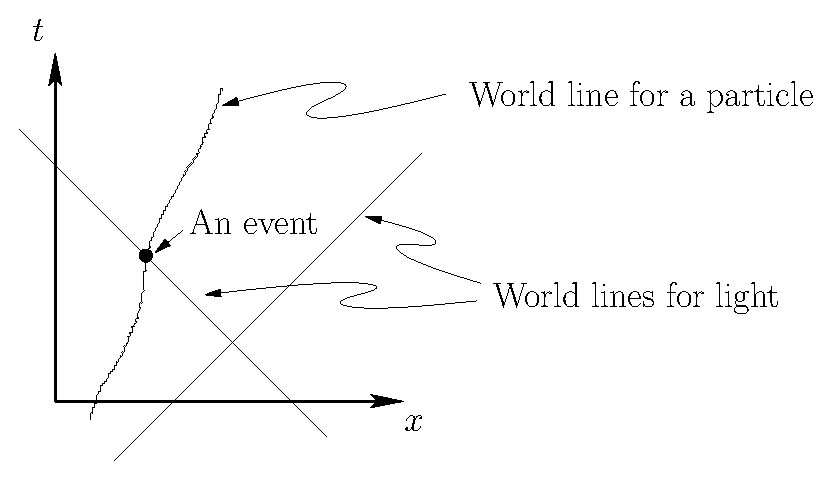
\includegraphics[width=3.5in]{relativistic_spacetime/spacetime1.eps}
\end{center}
\caption{A spacetime diagram with three world lines.  The two world lines for 
light have slopes $+1$ and $-1$.}
\label{fig:spacetime-example}
\end{figure}

Let's use a spacetime diagram to display the world lines of the
three-clock thought experiment of Ch.~\ref{chapter:relativityI},
Section~\ref{section:time-dilation} (see Fig.~\ref{fig:light-clocks}
from that section and Fig.~\ref{fig:worldlines1} in this section).
For example, put clock A at rest at $x = 0$ and clock B at rest at $x
= 0.60\units{lt-s}$.  The world lines for the stationary clocks A
and B are then vertical lines at $x = 0\units{lt-s}$ and $x =
0.60\units{lt-s}$.  Let clock C travel with speed $0.60c$ in the
positive $x$-direction.  Because $c = 1\units{lt-s/s}$, clock C
passes through $x = 0$ at time $t = 0\units{s}$, and it passes
through $x = 0.60\units{lt-s}$ at time $t = 1.0\units{s}$.  It has 
traveled a distance of $0.60\units{lt-s}$ in a time $1.0\units{s}$.
    
Notice in Fig.~\ref{fig:worldlines1} that we have labeled the world
line of clock C as the $t^\prime$ axis.  This is a general result: the
world line of a particular observer (say, someone traveling in a space
ship) is the $t^\prime$ axis for that observer.  This can be
understood by considering a person on a spaceship holding a ball. The
world line for the ball is the same as the world line of the ship and
person since they are all moving together.  From the perspective of
the astronaut, the ball remains right in front of him and isn't moving
anywhere, so it makes sense that that astronaut will say that the
location of the ball remains at $x^\prime = 0$.  And just as it is
true that the points where $x = 0$ in the unprimed frame define the
$t$-axis, so it is that the points where $x^\prime = 0$ in the primed
frame define the $t^\prime$-axis.
    
\begin{figure}[tbp]
\begin{center}
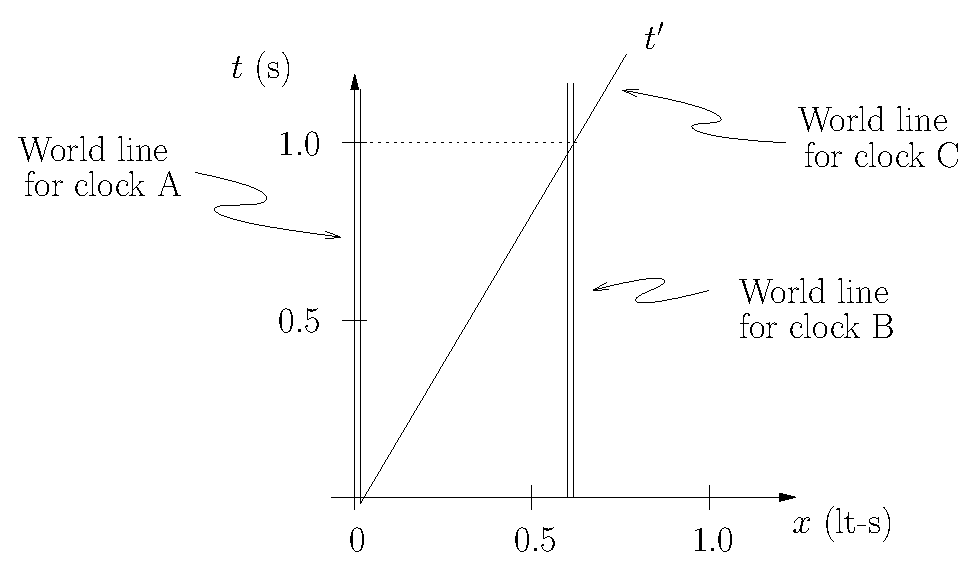
\includegraphics[width=4in]{relativistic_spacetime/worldlines1.eps}
\end{center}
\caption{World lines for the three clocks in the thought experiment
of Section~\ref{section:worldlines}}
\label{fig:worldlines1}
\end{figure}

Some comments are in order:
\begin{enumerate}
\item A world line is nothing more than a plot of time versus
position.  If you ever find yourself stumped about how to plot a
world-line, ask yourself: ``Where is the (whatever) at time $t=0$
(i.e., what is its initial $x$-coordinate)?  Where is it at time 
$t=1$?  At time $t=2$?  \dots''  Then simply plot those points 
and connect them.
\item The slope of a world line is simply $1/v$.  This comes from the
  standard relation: distance = speed $\times$ time, or equivalently, 
  $\Delta x= v \Delta t$.   So $\Delta t =
  \frac{1}{v}\Delta x$.  Practically, this means that if you have a ship
  moving at a speed of, say, $0.5c$, then the slope will be $1/ v$ or
  $2.0\units{s/lt-s}$.  When plotting a world line, this means that
  you go up 2 and over 1 (or over 0.5 and up 1).
\item Don't {\bf ever} forget --- nothing can travel faster than
light, so there should {\bf never} be a world line on a spacetime diagram
 with a
slope whose magnitude is less than 1.  
\item Remember: events are plotted as dots.
\item Label everything clearly.
\end{enumerate}

\begin{figure}[tbp]
\begin{center}
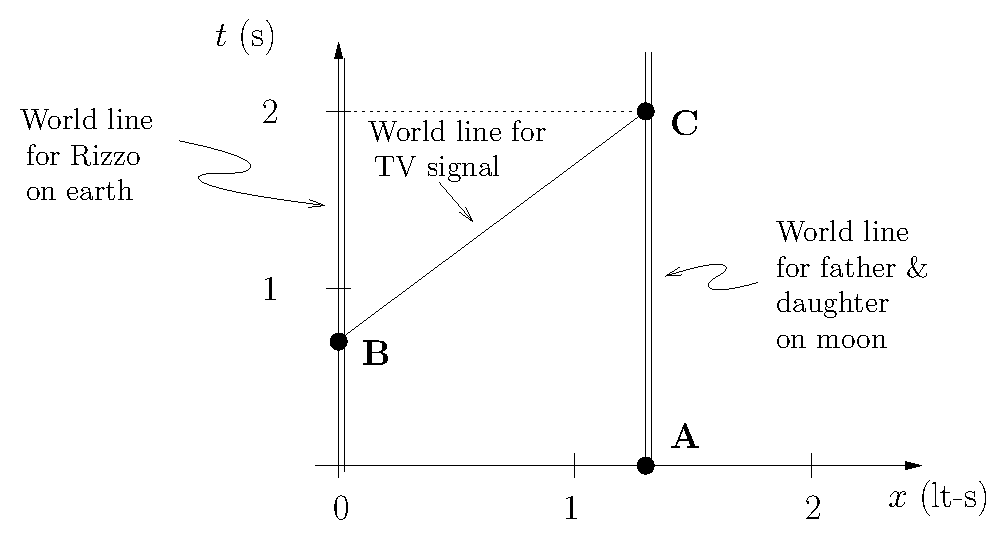
\includegraphics[width=4.2in]{relativistic_spacetime/worldlines2.eps}
\caption{Spacetime diagram for situation discussed in
  Examples~\ref{example:causality-intervals} and
  \ref{example:causality-intervals-diagram}}
\end{center}
\end{figure}

\begin{example}{Spacetime diagram corresponding to 
Example~\ref{example:causality-intervals}} Draw the spacetime diagram
  for the baseball scenario (Cubs losing the World Series) discussed
  in Example \ref{example:causality-intervals}, using the reference
  frame of the Earth/Moon.  Show the world lines for Anthony Rizzo, Jr.,
  the girl and her father, and the TV signal.  Also, show and label
  the following events: A --- girl sneezes, B --- Rizzo strikes out, and
  C --- girl and father see Rizzo striking out.  \solution The world
  lines for Rizzo and the girl/father are simply straight vertical lines
  since they aren't moving in the Earth-Moon reference frame.  If this
  isn't clear, then answer these questions: If we put the Earth at $x
  = 0$ at time $t = 0$, where is the Earth at time $t=1\units{s}$?
  Answer: still at $x = 0$.  At $t=2\units{s}$?  Answer: still at $x =
  0$.  The Earth's world line is nothing more that a set of points
  where $x$ is always zero.  As for the girl/father on the Moon, we
  already said in Example \ref{example:causality-intervals} that they
  are about $1.3\units{lt-s}$ away from the Earth.

We know from the problem that the girl/father see the strikeout
$2\units{s}$ after she sneezes.  So, if she sneezes at $t = 0$ (it is
arbitrary as to what we choose as the $t = 0$ time), then the TV
signal arrives at $t = 2\units{s}$.  It must have been sent from the
Earth at an earlier time, and since it travels at the speed of light,
then the world line for the TV signal is a $45^\circ$ line.  The only
thing left is to plot the three dots for the events.

Note that if you imagine a line between A and B, that line would 
have a slope with magnitude less than 1 (i.e., too shallow), 
indicating that nothing can travel between these two events, 
consistent with the result in Example 1 that the interval is space-like 
and the corresponding events can't be causally linked.
\label{example:causality-intervals-diagram}
\end{example}


\section[the relativity of simultaneity]{Ordering of events --- the 
relativity of simultaneity}

Every event has a set of space and time coordinates.  In Example
\ref{example:causality-intervals-diagram} above, we would say that the
event A (girl sneezes) occurs at time $t=0$ and location $x =
1.3\units{lt-s}$.  Similarly, we can determine the location and times
of events B and C, all as measured by observers in the Earth-Moon
reference frame. Let's add one more event to the scenario: let's say
that at time $t=0$, the pitcher Masahiro Tanaka, Jr., pitches the ball
toward Castro.  In Fig.~\ref{fig:father-daughter} we have added this event and
labeled it P.  In the Earth-Moon frame, we can say quite definitively
that A and P are simultaneous and come first, then B, then C.  Also, A
and C happen at the same location, and P and B happen at the same
location.

\begin{figure}[tbp]
\begin{center}
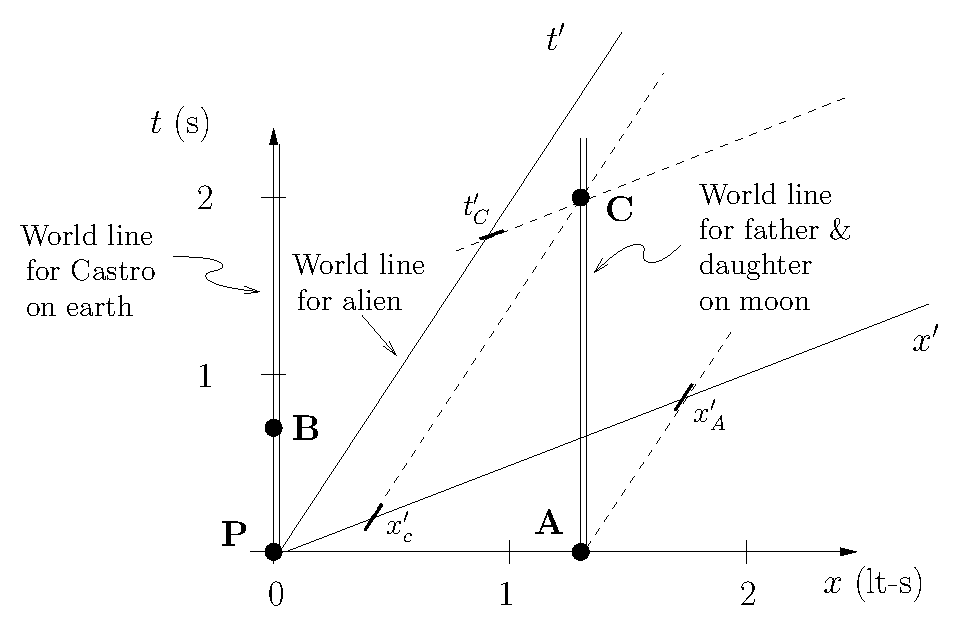
\includegraphics[width=4.3in]{relativistic_spacetime/worldlines3.eps}
\end{center}
\caption{Extension of spacetime diagram in Example
\ref{example:causality-intervals-diagram}.}
\label{fig:father-daughter}
\end{figure}
    
Special relativity helps us answer the following question: how does an
observer moving in a different reference frame view these same events?  We
won't worry here about the actual numerical values of $x^\prime$ and
$t^\prime$ (the position and time as measured by a different observer), but
we can say quite a lot about the ordering of events in space and time
by looking at the spacetime diagrams.


We have added another world line to Fig.~\ref{fig:father-daughter},
namely, the world line for a hypothetical alien whizzing past the
Earth just as the pitch is thrown.  This alien is monitoring the game
to try to understand human culture.  We assume the alien is traveling
at a speed $0.5c$; hence, the world line has a slope of 2.

We have already commented that the world line of an observer in a
primed frame is simply the $t^\prime$ axis for that frame, so we have
labeled the alien's world line $t^\prime$. But where should we put the
$x^\prime$-axis and what scale should we put on it?  It turns out that to
satisfy the invariance of the speed of light, we must draw the
$x^\prime$-axis at the same angle relative to the $x$-axis as the angle of
the $t^\prime$-axis relative to the $t$-axis. This means the slope of the
$x^\prime$-axis is equal to the speed $v$ of the primed frame relative to the
unprimed frame.
    
Recall that the $t^\prime$-axis represents points where $x^\prime =
0$.  It turns out that $x^\prime$ is constant along any line parallel
to the $t^\prime$-axis.  In other words, lines parallel to the $t^\prime$-axis
are equal-location lines for the primed frame of reference, just as
the $t$-axis and all lines parallel to it are each lines of equal
location for the unprimed frame of reference.  The same ideas work for
events on lines parallel to the $x$ or $x^\prime$ axes; events on a line
parallel to the $x$-axis are simultaneous in the unprimed frame, and
events on a line parallel to the $x^\prime$-axis are simultaneous in the
primed reference frame.
    
We can use these ideas to ``read off'' coordinates for events in
both reference frames.  As an example, let's look at event C in
Fig.~\ref{fig:father-daughter}.  We have already commented that in the
unprimed frame, its $x$ location is $1.3\units{lt-s}$ and its time
is $2\units{s}$.  The coordinates of this event in the alien's
reference frame are determined by drawing lines parallel to the
$x^\prime$ and $t^\prime$ axes (shown as dotted lines in
Fig.~\ref{fig:father-daughter}).  The intersections of these
construction lines with the opposing primed axis gives the $x_C$ and
$t_C$ coordinates. The rules for determining coordinates can be
summarized as follows:
\begin{enumerate}
\item To find $x_C$, draw a straight line through C parallel to the
$t$-axis and read off where it crosses the $x$-axis.  
\item To find $t_C$ draw a straight line through C parallel to the
$x$-axis and read off where it crosses the $t$-axis.  
\item To find $x_C^\prime$, draw a straight line through C parallel to
the $t^\prime$-axis and read off where it crosses the $x^\prime$-axis.
\item To find $t_C^\prime$, draw a straight line through C parallel to the
$x^\prime$-axis and read off where it crosses the $t^\prime$-axis.
\end{enumerate}

Using this type of construction, we can see that although events A and
C occur at the same place in the unprimed (Earth-Moon) reference
frame, event C happens to the left of the event A in the primed
(alien) reference frame.  This is easy to understand: the alien is far
from the Moon when event A happens, so A is far ``to the right,''
whereas the alien is close to the Moon when event C happens, so from
the alien's perspective, C isn't so far to the right, i.e.,
smaller $x^\prime$ coordinate.
    
    But what about the ordering of events in time?  We have commented
that the invariance of the spacetime interval says that if two
observers disagree about distances, then they will have to disagree
about time intervals as well.
    
\begin{boxittext}
{{\bf In preparation for class:} Look at the $t^\prime$ coordinates for events
P and A.  In the Earth-Moon reference frame, these events are simultaneous.
What about in the alien reference frame?
}
\end{boxittext}

We have said that any two events on a line parallel to the
$x^\prime$-axis are simultaneous in the primed frame of reference.
Similarly two events that lie on a line parallel to the $x$-axis are
simultaneous in the unprimed frame.  However two different events
cannot lie both on a line parallel to the $x$-axis and parallel to the
$x^\prime$-axis.  Thus two events that are simultaneous in one frame cannot
be simultaneous in the other frame.  We explore this idea in the
following example.

\begin{example}{Simultaneity is Relative}  
Einstein showed, with the following thought experiment, that two events
which occur at the same time but at different places in one frame,
occur at different times in another frame.

\begin{figure}[tbp]
\begin{center}
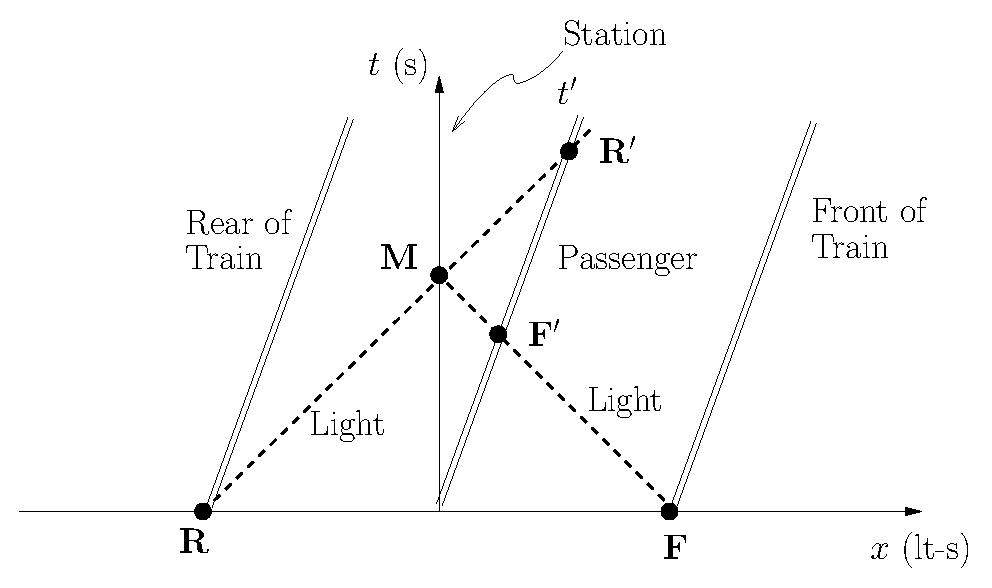
\includegraphics[width=4.2in]{relativistic_spacetime/worldlines4.eps}
\end{center}
\caption{Spacetime diagram for train of Example 
\ref{example:simultaneity}. (Light
world lines shown as dashed lines.)}
\label{fig:simultaneity}
\end{figure}

Imagine a train moving past a station.  By chance, lightning
happens to strike the front and back of the train at the same time
according to observers on the station platform.  Light pulses from
these strikes travel toward the middle of the train, where a passenger
observes their times of arrival.  Do the light pulses arrive
simultaneously or does one arrive before the other, and if so, which
one?
\solution
Use a spacetime diagram, Fig.~\ref{fig:simultaneity}, with the
station at rest in the unprimed frame and the train at rest in the
primed frame.  The $x$- and $x^\prime$-axes both lie along the track.
(Note:  this does {\bf not} mean that the $x$- and $x^\prime$-axes
are the same thing on a spacetime plot.  The $x^\prime$-axis is not
shown in Fig.~\ref{fig:simultaneity}, but remember that it is the mirror
image of the $t^\prime$-axis about a $45^\circ$ line; i.e., the angle
between the $t$- and $t^\prime$-axes is the same as the angle between
the $x$- and $x^\prime$-axes.)
The world line for the middle of the station is shown as the $t$-axis.

Because all parts of the train are at rest in the primed frame, we
draw the world lines for the front and the rear ends of the train
parallel to the $t^\prime$-axis.  Also, in
Fig.~\ref{fig:simultaneity}, we have chosen the world line for the
passenger riding in the exact middle of the train to be the
$t^\prime$-axis.  In the primed frame the front and rear world lines
are then equidistant from the passenger, by definition.

The lightning strikes occur at points R and F on the world lines of 
the rear and front of the train.  Because each strike represents an 
event and because these two events occur simultaneously in the 
station frame, R and F must be drawn on the same horizontal line.  
We arbitrarily choose this line to be at $t = 0$.

The light pulses produced by the lightning strikes travel with speed
$c = 1\units{lt-whatever per whatever}$ from the event F back toward
the passenger and from R forward toward the passenger.  The pulse from
F is represented by a world line of slope $-1$ and the pulse from R is
represented by a world line of slope $+1$.  Figure
\ref{fig:simultaneity} shows that the pulse from F arrives at the
passenger's world line (at F$^\prime$) earlier (i.e., at a smaller
value of $t^\prime$) than does the pulse from R, which arrives at
R$^\prime$.

The passenger must conclude that the front strike occurred before 
the rear strike because she is sitting in the middle of the train, 
equidistant from R and F, and she knows the light pulses must have 
taken the same time (in her frame) to reach her.  By the same 
argument, an observer on the station platform who was at the exact 
middle of the train at $t = 0$ when the strikes occurred, sees the 
pulses at the same time.  This is shown on the spacetime diagram 
by the fact that the world lines of the pulses cross the world line of 
the middle of the station at $x = 0$ (event M) at the same time.
\label{example:simultaneity}
\end{example}

\newpage

\section*{Problems}
\markright{PROBLEMS}

\begin{problem}
If two events are separated by a time-like interval in one
frame of reference, are they separated by a time-like interval in all
frames of reference?  Explain.
\end{problem}

\begin{problem}
A simple way of synchronizing two clocks at rest relative to one
another is to stand exactly halfway between them and emit light pulses
toward each of them at the same instant of time.  Each clock is then
set to 0 when the synchronizing pulse reaches it.
  \begin{enumerate}
  \item How does this scheme ensure that the clocks are started
    simultaneously?  
  \item On a spacetime diagram show the world lines of two
    clocks at rest in the unprimed frame of reference at $x = 0$ and at $x =
    L$, along with the world lines of two synchronizing light pulses that
    start from the midpoint and reach each of the two clocks at $t = 0.$
  \end{enumerate}
\label{prob:synchronizeB}
\end{problem}

\begin{problem}
  Events A, B, and C are shown on the spacetime diagram in
  Fig.~\ref{fig:spacetimeI}.
  \begin{figure}[h]
  \begin{center}
    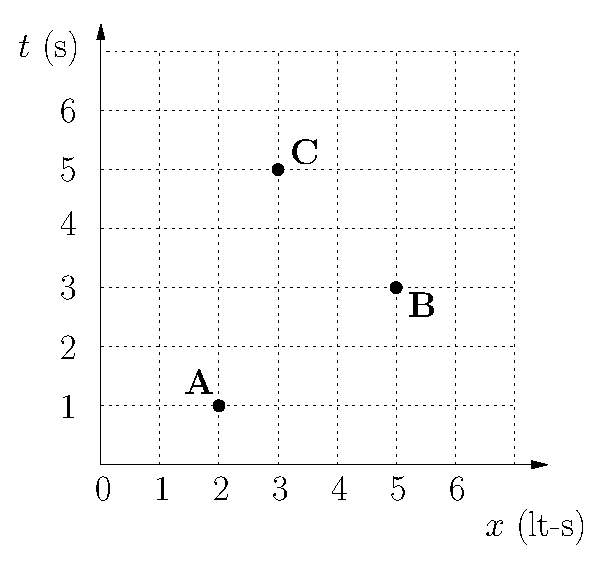
\includegraphics[width=2.8in]{relativistic_spacetime/p_spacetimeI.eps}
  \caption{Figure for Problem \ref{prob:spacetimeI}.}
  \label{fig:spacetimeI}
  \end{center}
  \end{figure}
  \begin{enumerate}
  \item Calculate the value of the squared interval for each pair of
    events, i.e., find $I^2_{AB}$, $I^2_{AC}$, and $I^2_{BC}$.  
  \item Label each interval as time-like, space-like, or light-like.  
  \item In the frame shown, event A occurs before B, which occurs before
    C.  Which pairs of events could have their time-order reversed
    (switching before and after) by choosing an appropriate reference
    frame?  
  \item In the frame shown, event B occurs to the right of C, which
    occurs to the right of A.  Which pairs of events could have their
    space-order reversed (switching left and right) by choosing an
    appropriate reference frame?  
  \item Which events could be a ``cause'' for which other events?
  \end{enumerate}
\label{prob:spacetimeI}
\end{problem}

\begin{problem}
Fig.~\ref{fig:spacetimeII} shows a spacetime diagram with seven straight lines
through the origin labeled with capital letters A through G.  Various
events are marked as points with small letters a through e.  The $x$-$t$
axes belong to the Earth's reference frame.

\begin{figure}[htbp]
\begin{center}
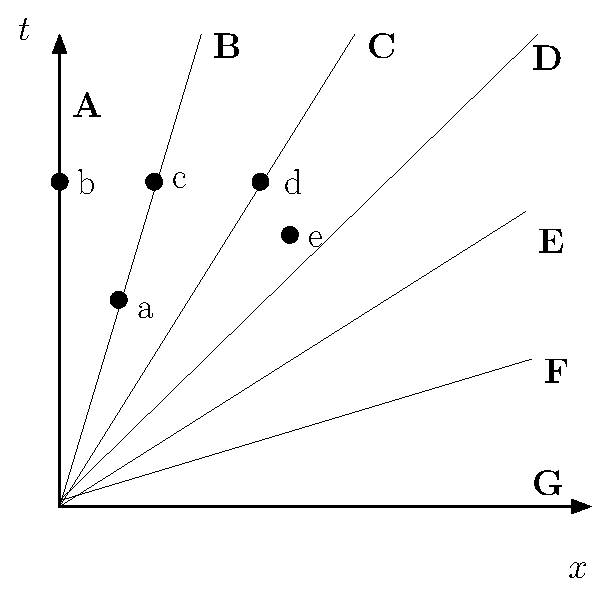
\includegraphics[width=2.5in]{relativistic_spacetime/p_spacetimeII}
\caption{Figure for Problem \ref{prob:spacetimeII}.}
\label{fig:spacetimeII}
\end{center}
\end{figure}
 
\begin{enumerate}
\item Which line is a world line of an object at rest relative to the Earth?
\item Which line is a world line of a spaceship traveling at speed  
$+0.3c$ relative to the Earth?
\item Which line is a world line of a light pulse emitted by the
spaceship as it passes the Earth? 
\item Which events happen simultaneously in the Earth frame?  
\item  Which events happen simultaneously in the spaceship frame?  
\item Which pairs of events are clearly separated by space-like
intervals?  Which are clearly separated by time-like intervals?
\end{enumerate}
\label{prob:spacetimeII}
\end{problem}

\begin{problem}
For Example \ref{example:simultaneity} in the text, show from
the spacetime diagram in Fig.~\ref{fig:simultaneity} that lightning
hit the front of the train at a negative value of $t^\prime$, but that
lightning hit the rear of the train at a positive value of $t^\prime$.
Use the rule for finding the $t^\prime$ coordinate of an event to
solve this problem.  [Hint: you might want to extend some of the axes
in the negative direction.]  
\end{problem}

\begin{problem}
Farmer Brown, at rest in his frame, carries a ladder through
a barn.  According to Farmer Brown, the ladder measures
$20\units{lt-ns}$.  According to observers at rest with respect
to the barn, Farmer Brown and his ladder are moving at a
speed $0.80c$ (alternately, Farmer Brown sees the barn 
moving at speed $0.80c$).  In the barn's frame, the
front door of the barn is at $x = 0 \units{lt-ns}$ and the back 
door is at $x = 16\units{lt-ns}$.
\begin{enumerate}
\item Calculate the length of the ladder as measured by
observers in the barn's reference frame.  According to
these observers, will the ladder fit within the barn?
\item Calculate the length of the barn as measured by
Farmer Brown.  According to Farmer Brown, will the ladder
fit within the barn?
\item Draw a careful spacetime plot for this situation,
with appropriate tick marks on the axes (labeled with
numbers).  Starting with the barn frame, draw world
lines for the entrance and exit of the barn (i.e., the
front and back doors).  Draw also world lines for the front and
back of the ladder (which is moving as viewed in the
barn frame).  The distance between the front and back of
the ladder in your plot should agree with your answer
to part (a), and the slopes of these lines should be
consistent with the known velocities.
\item Label the following events on your diagram:
A = front of ladder enters the barn; B = front of ladder
leaves the barn; C = back of ladder enters barn;
D = back of ladder leaves barn.  Determine the order
of these events in time as viewed from the barn's
reference frame.  Is this result consistent with your
answer to (a), i.e., whether or not the ladder fits in the
barn, according to barn-frame observers?  (Consider
whether the back of the ladder enters the barn before
or after the front of the ladder leaves the barn.)
\item Determine the order of events A, B, C and D as
viewed from Farmer Brown's reference frame.  Is this
result consistent with your answers to (b)?
\item Based on your answers for this problem, can you
see how relativistic time-ordering (i.e, the fact that
different observers do not necessarily agree on the
ordering of events in time) is necessarily linked with
length contraction?
\end{enumerate}
\label{prob:farmer}
\end{problem}

\newpage
\begin{figure}[!h]
\[ 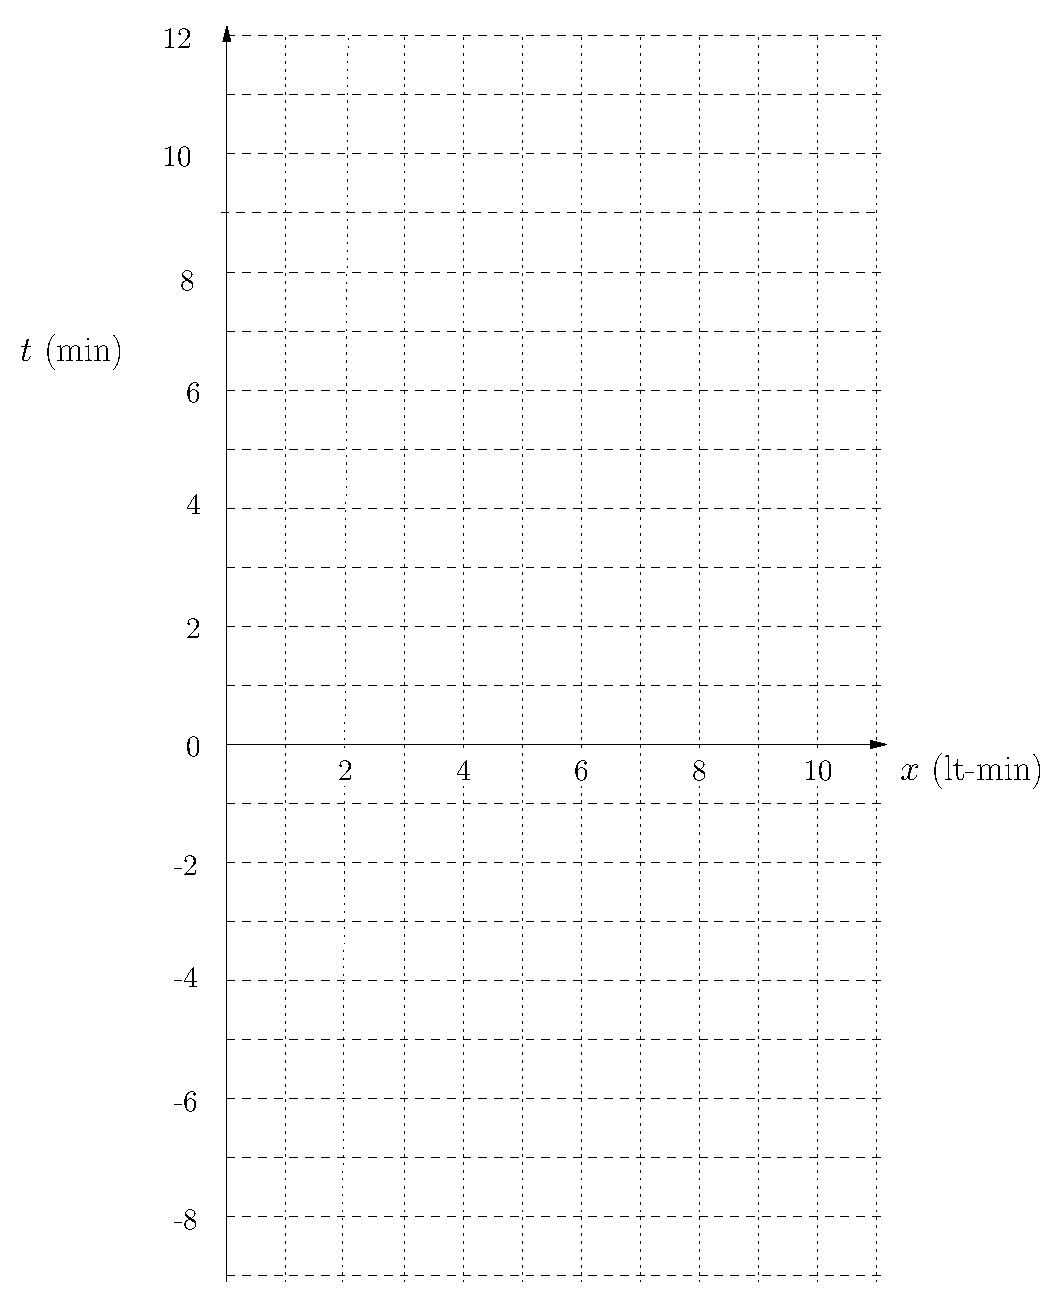
\includegraphics[width=5.5in]{relativistic_spacetime/p_solar_flare.eps} \]
\caption{Figure for Problem \ref{prob:solar_flare}.}
\end{figure}

\newpage

\begin{problem}
The Earth is $8\units{lt-min}$ from the Sun.  An astronomer on Earth,
looking through a telescope, notices the sudden appearance of a giant
solar flare on the Sun's surface.  At precisely that instant (when the
astronomer detects the flare), a Klingon space ship whizzes over his
head at speed $0.8c$, heading straight for the Sun.
\begin{enumerate}
\item On the facing page, construct a spacetime diagram for this situation.  
  Label the following three events: {\bf A}: Klingon ship hits Sun, 
  {\bf B}:  flare occurs on Sun, and {\bf C}: Klingon ship passes Earth.  
  (Note that event B is the occurrence of the flare {\em on\/} the Sun, 
  not the detection of the flare by an astronomer on Earth.)
\item Order the events A, B, C, from earliest to latest, according to
  Earth-based observers.
\item Calculate the time intervals $\Delta t$ between each pair of
  events (AB, AC, and BC), according to Earth observers.
\item Calculate the interval $\Delta t^\prime_{BA}$ between events B
  and A, but now according to Klingon ship observers.
\item Classify each of the intervals as space-like, time-like or
  light-like.
\end{enumerate}
\label{prob:solar_flare}
\end{problem}

% \begin{problem}
% A cosmic ray particle moving down toward Earth at speed $0.99c$ decays
% $2.0\units{$\mu$s}$ after it was produced as measured in the frame in
% which the particle is at rest.
% \begin{enumerate}
% \item Represent the birth and decay of the particle on a spacetime
%   diagram.
% \item In the cosmic ray's rest frame the Earth is moving toward it.
%   In this frame, how far, in light-$\mu$s, did the Earth travel during
%   the particle's lifetime?
% \item Observers in the Earth's frame see the particle coming down
%   toward Earth.  How long did the particle live according to these
%  observers and how far did it travel?
% \end{enumerate}
% \label{prob:cosmic_ray}
% \end{problem}

\begin{problem}
Two spacecraft, {\em Aaaak} and {\em Blech}, are carrying aliens from 
the planet Zortox to Earth.  Both spacecraft are traveling
at a speed of $0.6c$ relative to the Earth, with {\em Aaaak} in
front.  In the Earth's frame, {\em Aaaak} and {\em Blech} are
a distance $8.0\units{lt-s}$ apart. 
At the moment that {\em Aaaak} passes Earth, the Zortoxians aboard {\em Aaaak} 
dump its garbage.  At a time $10.0\units{s}$ later 
(as measured by earthlings) {\em Blech} dumps its garbage.  
\begin{enumerate}
\item Draw a spacetime diagram in Earth's frame that includes 
worldlines for Earth, {\em Aaaak}, and {\em Blech}.  Indicate and label 
the events corresponding to the garbage dumps.
\item How far has {\em Blech} traveled during the $10.0\units{s}$ 
between the two garbage dumps measured by earthlings?
\item What is the distance between the two garbage dump events measured by 
earthlings?
\item What is the distance between the two garbage dump events 
measured by the Zortoxians on board their ship?
\item Calculate the time interval between garbage dump events measured by 
the Zortoxians on board their ship.
\end{enumerate}
\label{prob:two_ships}
\end{problem}

%\begin{problem}
%Two spacecraft ({\em Aaaak} and {\em Blech}) carrying aliens from 
%the planet Zortox are traveling toward  Earth (with {\em Aaaak} in front) 
%at a speed of $0.6c$ relative to the Earth.  In the Earth's frame of 
%reference {\em Aaaak} and {\em Blech} are $8.0\units{lt-s}$ apart. 
%At the moment they pass Earth, the Zortoxians aboard {\em Aaaak} 
%dump its garbage, and $10.0\units{s}$ later 
%(as measured by earthlings) {\em Blech} dumps its garbage.  
%\begin{enumerate}
%\item Draw a spacetime diagram in Earth's frame that includes 
%worldlines for Earth, {\em Aaaak}, and {\em Blech}.  Indicate and label 
%the events corresponding to the garbage dumps.
%\item How far has {\em Blech} traveled during the $10.0\units{s}$ 
%between the two garbage dumps measured by earthlings?
%\item What is the distance between the two garbage dump events measured by 
%earthlings?
%\item What is the distance between the two garbage dump events 
%measured by the Zortoxians on board their ship?
%\item Calculate the time interval between garbage dump events measured by 
%the Zortoxians on board their ship.
%\end{enumerate}
%\label{prob:two_ships}
%\end{problem}


\newpage

\begin{problem}
A train of rest length $40\units{lt-ns}$ moves along the
tracks at $0.8c$ and is struck by two lightning bolts.  One bolt hits
the front of the train and the other hits the back.  According to
observers  on the tracks the bolts are simultaneous.
\begin{enumerate}
\item How far apart did the lightning bolts strike according to 
observers on the tracks?  
\item According to riders on the train, how much time passed between the
striking of the lightning bolts?  
\item According to riders on the train, which lightning bolt 
struck first? 
\end{enumerate}
\end{problem}

\begin{problem}
Joe holds and lights a sparkler, and one minute later, it goes
out.  Cheri, riding in a rocket past these events, notes that, as
measured in her frame, the sparkler burned for 100 seconds.
\begin{enumerate}
\item How far apart in Cheri's frame did these two events (lighting
and going out) occur? 
\item As measured by Cheri, how far did the lit sparkler travel, and
how fast was it moving?  
\item As measured by Joe, how fast was Cheri traveling during the one
minute of sparkler light, and how far did she travel?
\end{enumerate}
\label{prob:sparkler}
\end{problem}

\newpage

\begin{problem}
The spacetime diagram in the figure shows the world lines of the Earth,
a star, and a rocket, as well as several labeled events.
\begin{figure}[!h]
\begin{center}
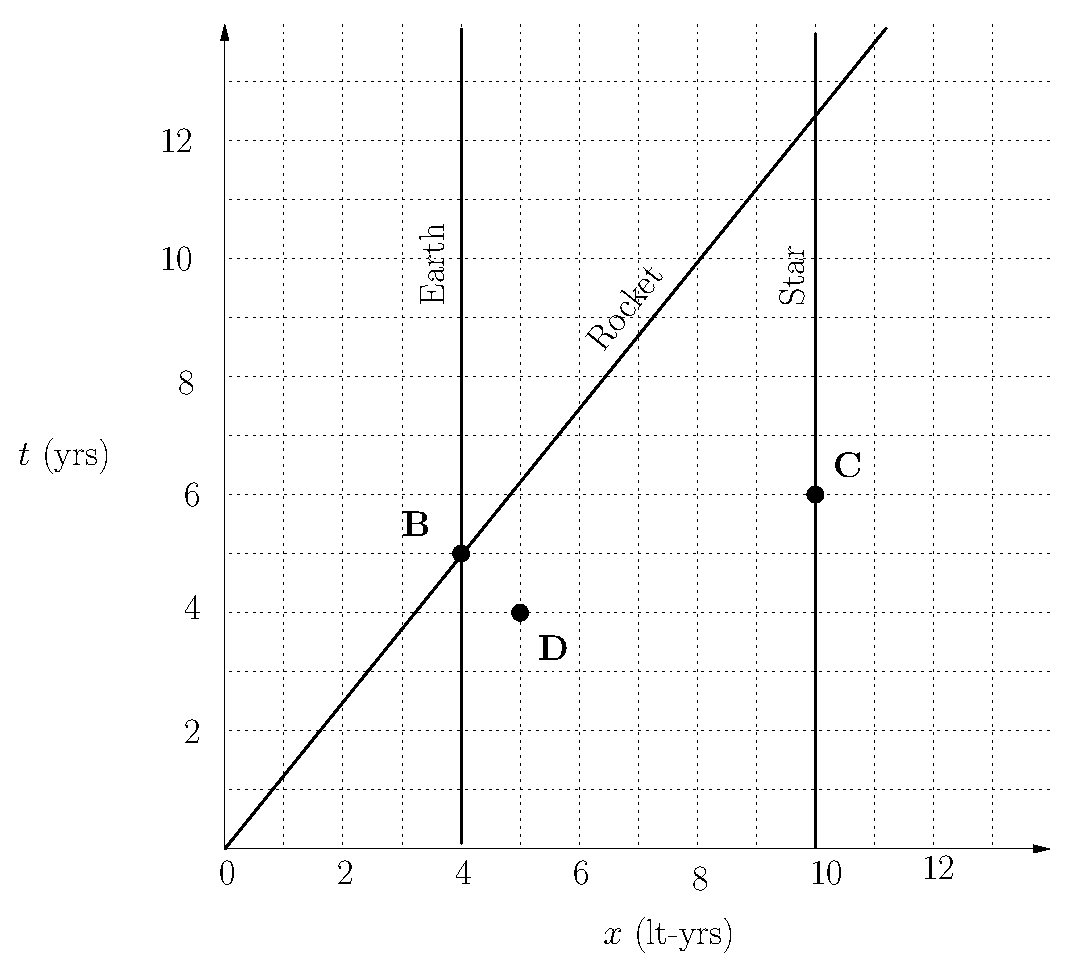
\includegraphics[width=3.68in]{relativistic_spacetime/p_spacetimeIII.eps}
\end{center}
\caption{Figure for Problem \ref{prob:spacetimeIII}.}
\end{figure} 
\begin{enumerate}
\item On the diagram, label as ``A'' the event ``Rocket arrives
at Star.''
\item Determine the speed of the Rocket, as measured by Earth
observers.
\item Determine the time between passing the Earth and passing the
Star, as measured by Rocket observers.
\item Determine the distance between the Earth and the Star, as
measured by Rocket observers.
\item Draw the world line of a lost satellite passing the Earth at the
same time as the Rocket, but going away from the Star at a speed that
is $\frac{1}{2}$ of the Rocket speed (as determined by Earth
observers.)  Label this line ``Satellite.''
%\item Determine the speed of the satellite as measured by Rocket observers.
%This part removed in 2011 when velocity transformations moved to mom/energy
%chapter.
\item Order the events A, B, C, D, from earliest to latest, as
observed in the Earth-Star reference frame.
\item Order the events A, B, C, D, from earliest to latest, as
observed in the Rocket reference frame.  
\item In some reference frame, the events C and D are simultaneous.
In that frame, what is the distance between events C and D?
\item Explain why no one could ever measure the proper time between
events C and D.  
\end{enumerate}
\label{prob:spacetimeIII}
\end{problem}
